\documentclass{article}
\usepackage{graphicx} % Required for inserting images
\usepackage{derivative}
\usepackage[T2A]{fontenc}
\usepackage[utf8]{inputenc}
\usepackage[english, russian]{babel}
\usepackage{amsfonts}
\usepackage{amsmath}
\usepackage[left=2cm,right=2cm,
    top=2cm,bottom=2cm,bindingoffset=0cm]{geometry}
\setlength\parindent{1.5em}
\DeclareMathOperator{\grad}{grad}
\DeclareMathOperator{\lagr}{\mathcal{L}}


\title{Домашнее задание 1 (тервер)}
\author{Андрей Зотов}
\date{Сентябрь 2023}

\begin{document}

\maketitle

\section*{Задача 1}
{\bf Ответ: } $0.44$.
\\
\\
{\bf Решение.} 
\par
Пусть $A$ - событие <<увидеть рекламу в СМИ>>, $B$ - событие <<увидеть рекламу в соцсетях>> и $C = A\cup B$ - событие <<увидеть рекламу в соцсетях или в СМИ>>. Тогда $P(C)=P(A\cup B)=P(A)+P(B)-P(AB)$ и т.к. события $A$ и $B$ независимы, то $P(AB)=P(A)P(B)$. Поэтому $P(C)=P(A)+P(B)-P(A)P(B)=0.2+0.3-0.06=0.44$.
\section*{Задача 2}
{\bf Доказательство.}
\par
Т.к. $A$ и $B$ независимы, то $P(AB)=P(A)P(B)$. Также воспользуемся тем, что $P(\bar X)=1 - P(X)$ для любого события $X$.
\\
\\
{\bf a)} Т.к. $\bar A\bar B = \overline{A \cup B}$, то $P(\bar A\bar B)=P(\overline{A \cup B}) = 1 - P(A \cup B) = 1 - P(A) - P(B) + P(AB) = 1 - P(A) - P(B) + P(A)P(B)=(1-P(A))(1-P(B))=P(\bar A)P(\bar B)$. Что и требовалось доказать.
\\
\\
{\bf б)} Т.к. $A=AB\sqcup A\bar B$, то $P(A)=P(AB)+P(A\bar B)\Rightarrow P(A\bar B)=P(A)-P(AB)=P(A)-P(A)P(B)=P(A)(1-P(B))=P(A)P(\bar B)$. Что и требовалось доказать.
\section*{Задача 3}
{\bf Решение.} 
\par
Рассмотрим правильный тетраэдр, у которого первая грань раскрашена в красный цвет, вторая - в зеленый, третья - в синий, а четвертая в красный, зеленый и синий цвета (т.е. четвертая грань разделена на 3 области, каждая из которых покрашена в свой цвет).
\par
Пусть событие $A$ - <<после подбрасывания тетраэдр приземлился на грань с красным цветом>>, событие $B$ - <<после подбрасывания тетраэдр приземлился на грань с зеленым цветом>> и событие $C$ - <<после подбрасывания тетраэдр приземлился на грань с синим цветом>>. При этом приземление на любую из четырех граней считаем равновероятным элементарным исходом. Т.е. всего в нашем пространстве 4 элементарных исхода с вероятностью $1/4$ каждый. 
\par
Тогда $P(A)=P(\text{<<Тетраэдр приземлился либо на первую грань, либо на четвертую>>})=1/4+1/4=1/2$, аналогично $P(B)=1/2$ и $P(C)=1/2$. При этом $P(AB)=P(\text{<<Тетраэдр приземлился на 4ю грань>>})=1/4$, т.е. $P(AB)=P(A)P(B)=1/2\cdot 1/2=1/4$, что означает что события $A$ и $B$ независимы. Аналогично независимы события $A$ и $C$ и события $B$ и $C$.
\par
Однако $P(ABC)=P(\text{<<Тетраэдр приземлился на 4ю грань>>})=1/4\neq P(A)P(B)P(C)=1/8$. Таким образом 3 события $A,B,C$ попарно независимы, но не являются независимыми в совокупности. Что и требовалось показать.
\section*{Задача 4}
{\bf Ответ: } предпочтителен второй вариант (сильный - слабый - сильный), вероятность победы тогда будет $pq(2-q)$.
\\
\\
{\bf Решение.} 
\par
Найдем вероятность $p_1$ события $A_1$ <<Игрок выигрывает в двух партиях подряд в варианте 1>>. Событие $A_1$ состоит из 3-х элементарных исходов:
\begin{itemize}
    \item $\omega_1=\text{(Выиграл слабого; Выиграл сильного; Выиграл слабого)}\Rightarrow$ вероятность $P(\omega_1)=p\cdot q\cdot p$ (перемножаем вероятности, т.к. результаты партий независимы в совокупности);
    \item $\omega_2=\text{(Выиграл слабого; Выиграл сильного; Проиграл слабому)}\Rightarrow P(\omega_2) = p\cdot q \cdot (1 - p)$;
    \item $\omega_3=\text{(Проиграл слабому; Выиграл сильного; Выиграл слабого)}\Rightarrow P(\omega_3)=(1-p) \cdot q \cdot p$.
\end{itemize}
\par
Таким образом $p_1=P(A_1)=P(\omega_1\sqcup\omega_2\sqcup\omega_3)=pqp+pq(1-p)+(1-p)qp=pq(p+1-p+1-p)=pq(2-p)$. Аналогично находим вероятность $p_2$ события $A_2$ <<Игрок выигрывает в двух партиях подряд в варианте 2>>: $p_2=P(A_2)=pq(2-q)$.
\par
Отсюда получаем, что если $pq>0$, то из того, что $q < p$ следует $2 - q > 2 - p$ и поэтому $p_2=pq(2-q) > pq(2-p)=p_1$. Т.е. в этом случае второй вариант предпочтительней, а вероятность выиграть равна $pq(2-q)$. Если же $pq=0$, то $q=0$ и $p>0$ (по условию $q < p$), в этом случае в обоих вариантах вероятность выигрыша равна 0, что в принципе не противоречит формуле выигрыша для первого случая $pq(2-q)$, т.к. она обращается в 0 при $q=0$. Т.е. при любых допустимых значениях $p$ и $q$ можно придерживаться второго варианта для максимизации вероятности выигрыша.
\section*{Задача 5}
{\bf Ответ: } $\frac{31}{72}$.
\\
\\
{\bf Решение.} 
\par
Пусть $x$ - время прихода Алисы, а $y$ - время прихода Боба, при этом будем, считать момент 11:00 эквивалентным моменту $t=0$, а момент 12:00 эквивалентным моменту $t=1$. Тогда пространство элементарных исходов $\Omega$ будет состоять из точек квадрата $[0, 1]\times[0, 1]$ в прямоугольной системе координат $Oxy$.
\par
Если первым приходит Алиса в момент $x\in[0, 1]$, то у Боба есть в лучшем случае 10 минут (1/6 часа), чтобы встретиться, т. е. встреча будет возможна, если $y\in [x, \min(x+1/6,1)]$. Если же первым приходит Боб в момент $y\in[0,1]$, то у Алисы есть в лучшем случае 20 минут (1/3 часа), чтобы встреться, т. е. встреча будет возможна, если $x\in [y, \min(y+1/3,1)]$. Поэтому на рисунке ниже изображена закрашенная зеленым область квадрата $[0, 1]\times[0, 1]$, состоящая из точек (элементарных исходов) относящихся к событию $E$ <<Алиса и Боб встретились>>.
\\
{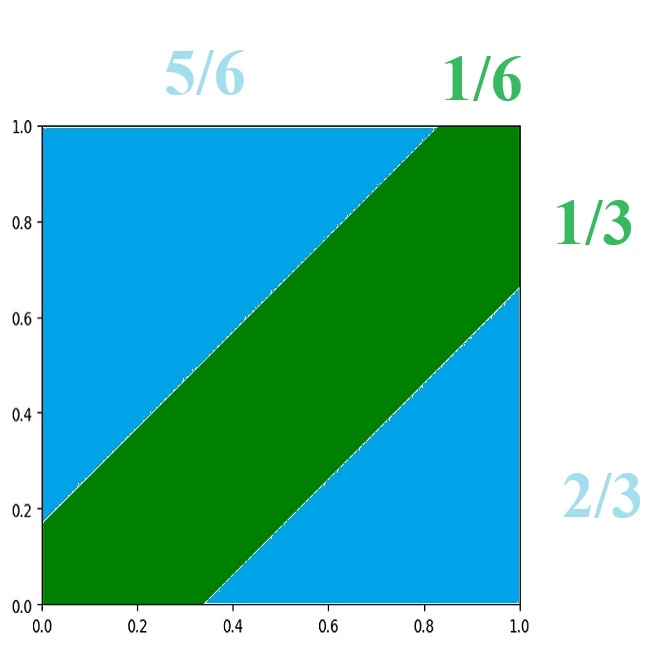
\includegraphics[scale=0.4]{img/img1.jpg}}
\par
Т.к. площадь квадрата $[0, 1]\times[0, 1]$ равна $1$, то площадь зеленой области и есть вероятность события $E$. Заметим, что событие $\bar E$ — это два синих треугольника на рисунке выше. Их площадь, т.е. вероятность $\bar E$ будет $P(\bar E)=1/2*(2/3)^2+1/2*(5/6)^2=\frac{41}{72}$, поэтому $P(E)=1-P(\bar E)=1-\frac{41}{72}=\frac{31}{72}$.
\section*{Задача 6}
{\bf Ответ: } a) $\frac{1}{2}$; б) $1-\frac{\pi}{4} \approx 0.2146$.
\\
{\bf Решение.} 
\par
{\bf a)} В этой задаче элементарным исходом является случайная точка $(x,y,z) \in [0, 1]\times[0, 1]\times[0, 1]$, где $x,y,z$ - случайные длины отрезков. Т.е. пространство $\Omega$ - это единичный куб в прямоугольной системе координат $Oxyz$. Чтобы отрезки с длинами $(x,y,z)$ могли образовать треугольник необходимо и достаточно чтобы выполнялись неравенства треугольника: $x + y > z,\ x + z > y,\ y + z > x$. Эти неравенства определяют область, вложенную в единичный куб, объем которой и будет искомая вероятность. Все неравенства линейные, поэтому границы искомой области определяются тремя плоскостями и гранями единичного куба. Найдем эти плоскости - достаточно предъявить для каждой плоскости 3 точки, не лежащие на одной прямой: 
\begin{itemize}
    \item Плоскость $x + y = z$ проходит через вершины куба $O=(0,0,0),\ A_1=(1, 0, 1),\ A_2=(0, 1, 1)$;
    \item Плоскость $x + z = y$ проходит через вершины куба $O=(0,0,0),\ B_1=(1, 1, 0),\ B_2=(0, 1, 1)$;
    \item Плоскость $y + z = x$ проходит через вершины куба $O=(0,0,0),\ C_1=(1, 1, 0),\ C_2=(1, 0, 1)$.
\end{itemize}
\par
Как можно заметить $B_2=A_2,\ A_1=C_2,\ B_1=C_1$. Обозначим также вершину куба $D=(1,1,1)$. Ниже наглядное изображение куба с отмеченными точками.
\\
{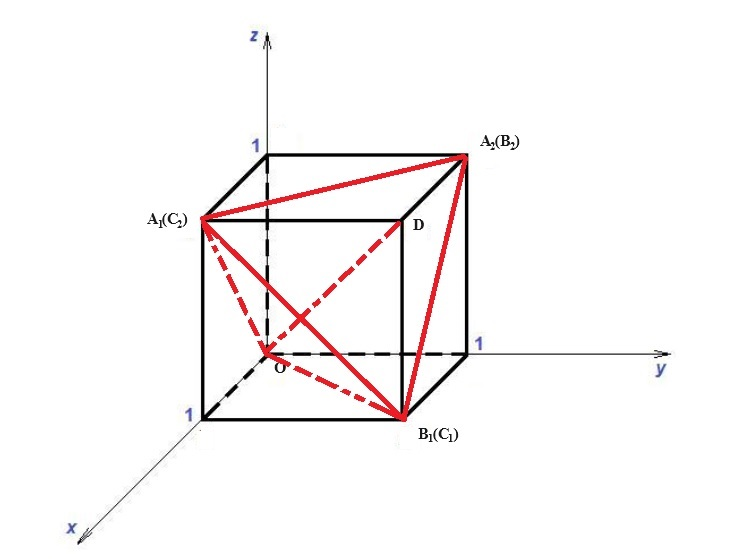
\includegraphics[scale=0.6]{img/img2.jpg}}
\\
\par
Таким образом событие $E$ <<отрезки с длинами $x,y,z$ образуют треугольник>> - это многогранник $OA_1A_2B_1D$ (он в частности содержит диагональ куба $OD$ - элементарные исходы соответствующие правильным треугольникам). Этот многогранник состоит из двух тетраэдров $T_1=OA_1A_2B_1$ и $T_2=DA_1A_2B_1$. При этом заметим, что событие $\bar E$ состоит из трех тетраэдров, таких же по объему как $T_2$ (в силу симметрии), но примыкающих к осям $Ox,\ Oy,\ Oz$, т.е. $P(E)=1-P(\bar E)=1-3\cdot V(T_2)$. Поэтому достаточно найти объем тетраэдра $T_2$. 
\par
Т.к. тетраэдр $T_2$ прямоугольный (все плоские углы трехгранного угла $D$ прямые), то его объем будет равен $V(T_2)=\frac{1}{6}\cdot abc$, где $a,b,c$ - длины ребер трехгранного угла $D$. В нашем случае $a=b=c=1$ и поэтому $V(T_2)=\frac{1}{6}\Rightarrow P(E)=1-3\cdot\frac{1}{6}=\frac{1}{2}$.
\par
{\bf б)} Рассмотрим произвольный остроугольный треугольник со сторонами $x,y,z$. Пусть напротив стороны $z$ лежит острый угол $\alpha$, тогда по теореме косинусов $x^2+y^2-2xy\cos \alpha = z^2$ или $\cos \alpha = \frac{x^2+y^2-z^2}{2xy}$, т.к. $0< \alpha < \frac{\pi}{2}$, то $\cos \alpha > 0$, т.е. $x^2+y^2-z^2 > 0$. 
\par
Таким образом, если треугольник остроугольный, то верно, что
\begin{equation}\label{eq1}
 \begin{cases}
   x^2+y^2-z^2 > 0\\
   x^2+z^2-y^2 > 0\\
   y^2+z^2-x^2 > 0\\
   x > 0,\ y > 0,\ z > 0
 \end{cases}
\end{equation}
\par
Верно и обратное: если для некоторых $x>0,y>0,z>0$ выполняется $(\ref{eq1})$, то из отрезков с длинами $x,y,z$ можно составить остроугольный треугольник. Действительно, если $x > 0,\ y > 0,\ z > 0$ и $x^2+y^2 > z^2$, то $x^2+2xy+y^2 > z^2 \Rightarrow (x+y)^2 > z^2\Rightarrow x + y > z$ (тут важно, что $x,y,z$ строго положительные величины). Получаем, что из $(\ref{eq1})$  вытекают все три неравенства треугольника, поэтому $x,y,z$ образуют треугольник. При этом косинусы всех углов положительные, т.е. углы острые.
\par
Таким образом $(\ref{eq1})$ - это критерий существования остроугольного треугольника со сторонами $x > 0,\ y > 0,\ z > 0$.
\par
По аналогии с пунктом а) нужно понять какую фигуру образует система $(\ref{eq1})$ в пересечении с единичным кубом. Заметим, что при $z\in [0, 1]$ уравнение $z^2-x^2-y^2=0$ - это круговой конус с вершиной в точке $(0,0,0)$ и осью вдоль $Oz$. При этом в единичный куб попадает только четвертая часть этого конуса (т.к. $x>0, y>0$ - это только один квадрант плоскости $Oxy$). Два других уравнения системы $(\ref{eq1})$ дают два аналогичных конуса с осями вдоль $Ox$ и $Oy$. 
\par
Получили, что внешность этих трех конусов (которая кстати содержит диагональ $OD$), лежащая внутри единичного куба, и будет событие $E$ <<отрезки с длинами $x,y,z$ образуют остроугольный треугольник>>. Заметим, что событие $\bar E$ — это внутренность трех четвертинок конусов, которые были рассмотрены выше. 
\par
Формула объема конуса $V_{con}=\frac{1}{3}\cdot h \cdot \pi r^2$, где $h$ - высота конуса, а $r$ - радиус основания. В нашем случае $h=r=1$, поэтому $P(E)=1-P(\bar E)=1-\frac{3}{4}\cdot V_{con} = 1 - \frac{3}{4}\cdot\frac{\pi}{3}=1-\frac{\pi}{4}$.
\\
\\
{\bf P.S.}
\par
Красивая двумерная модель вероятностного пространства для задачи 6 описана в работе <<Г. Корбулон, Каких больше – острых или тупых?, Квант, 2015, номер 3, 41–42>>
\\
https://www.mathnet.ru/rus/kvant1589
\\
\par
Цитата: <<Можно считать так. Взять три отрезка случайной длины и попробовать из них сложить треугольник – для этого нужно, чтобы длина самого длинного из них была все же меньше, чем сумма
двух оставшихся. Чтобы не возиться с сантиметрами и футами или парсеками с ангстремами, за единицу длины возьмем длину самого длинного отрезка. Тогда длины двух оставшихся отрезков ($x$ и $y$) будут числами меньше единицы, а условие, что из этих отрезков можно сложить треугольник, запишется так: $x + y > 1$. Если отложить $x$ и $y$ по осям, то диагональ квадрата $x + y = 1$ (красная линия) разделит его пополам (рис. 1), т.е. в половине возможных
случаев из трех случайно взятых отрезков нельзя вообще сложить треугольник.
{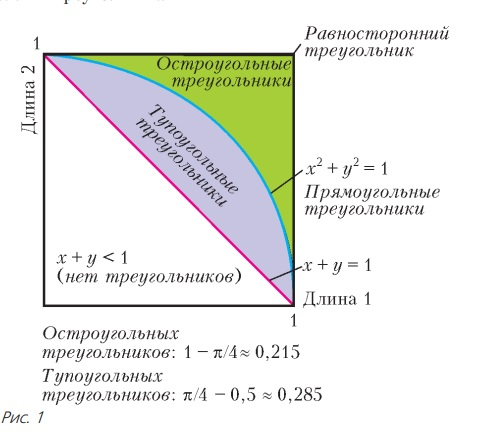
\includegraphics[scale=0.6]{img/img3.jpg}}
\par
Если учесть, что у прямоугольных треугольников $x^2 + y^2 = 1$ (дуга окружности, синяя линия), получим области «острых» и «тупых» треугольников. Площадь фиолетового сегмента равна $\frac{\pi}{4}-0.5\approx0.285$, а площадь зеленой области равна $1-\frac{\pi}{4}\approx 0.215$>>.

\end{document}
